\documentclass{article}

\usepackage[backend=bibtex, bibencoding=ascii]{biblatex}
\bibliography{wikipedia, mendeley}

\usepackage{amsmath}
% \usepackage[ngerman]{babel}
\usepackage[utf8]{inputenc}
\usepackage{amssymb}
\usepackage{amsxtra}
\usepackage{listings}
\usepackage{graphics}
\usepackage{url}
\usepackage{svg}
\usepackage{enumitem}

\usepackage{todonotes}

% \usepackage{marginnote}
% \reversemarginpar

\newcommand{\refchapter}[1]{Chapter~\ref{#1}}
\newcommand{\refsec}[1]{Section~\ref{#1}}
\newcommand{\refeqn}[1]{Equation~(\ref{#1})}
\newcommand{\reffig}[1]{Figure~\ref{#1}}

\setlength{\parskip}{1em}

\newcommand{\bluetext}[1]{%
  \marginnote{\color{gray}#1}} % \small\itshape
	
\newcommand{\annotation}[1]{%
%\uppercase{\bluetext{#1}}}
	\bluetext{#1}}

\title{
{\bf \scriptsize RHEINISCH-WESTFÄLISCHE TECHNISCHE HOCHSCHULE AACHEN} \vspace{2cm} \\
{\large Seminar on Numerical Libraries} \vspace{1em}\\
QUADRATURE \vspace{1em}\\
 }
\author{
Tobias Schürg
}

%\date{\includegraphics[height=2cm]{figures/logo_stce}}

\begin{document}

\lstloadlanguages{[ISO]C++}
\lstset{basicstyle=\small, numbers=left, numberstyle=\footnotesize,
  stepnumber=1, numbersep=5pt, breaklines=true, escapeinside={/*@}{@*/}}


\pagestyle{headings}

\maketitle


\begin{abstract} This paper gives an introduction to numerical quadrature. 
Besides common approaches such as the Midpoint rule, Simpson's rules and 
Gaussian quadrature an overview of the routines, included in 
numerical libraries, is given. The GNU Scientific Library and the NAG 
Numerical Library are considered as representative for this purpose. 
\smallskip
The aim of this work is to give an overall introduction and 
thus to be a central entry point when considering numerical integration. 

\bigskip \noindent \textbf{Keywords.} Composite Rule, Integration, Gaussian 
Quadrature, GSL, Midpoint Rule, Monte-Carlo Quadrature, NAGlib, Newton-Cotes 
Quadrature, Numerical Integration, Quadrature, Trapezoid Rule, 

\end{abstract}

\newpage

\tableofcontents 


\section{Introduction}

Quadrature itself is a historical term and originally meant 
determining the area of a plane figure by constructing a square that 
has the same area as the given figure. \emph{Squaring the circle}, also known as quadrature of the circle, is beside \emph{doubling the cube} and \emph{trisecting the angle} the most famous of the three classical problems in Greek mathematics which was extremely influential in the development of geometry and calculus.

Quadrature is now more or less a synonym for integration, especially as applied to one-dimensional integrals and is generally used to mean numerical integration \cite{Wiki_Integration}.

If $f(x)$ is a continuous real-valued function defined on a closed interval $[a, b]$, the area below the graph can be exactly computed with the antiderivative $F(x)$ of $f(x)$, for which $f = F'$ applies. The value of the integral on the closed interval is then determined by formula (\ref{integral}). \cite{HeuserAnalysis} 

\begin{equation} \label{integral} 	
\int_a^b\! f(x)\, dx = F(b) - F(a) 
\end{equation}



\subsection{Problem Description}
There are cases when an exact mathematical integration is not available (or needed) and a numerical approach becomes useful. Then, approximating a definite integral from few values of the integrand is of central interest. There are several cases when this problem occurs, the most important are described next.

\subsubsection{The integrand is partially unknown}
In many situations, such when points are obtained by sampling, the integrand $f(x)$ may be known only at a finite set of points. Of course, the data points can be interpolated by a polynomial of which an antiderivative is known and is thereby integratable but without background knowledge about the origin, this interpolated polynomial might increase the error. 

\subsubsection{The antiderivative is unknown}
There are cases when the antiderivative is unknown or can only be estimated symbolically but with much more effort. An example of a function which can not be calculated easily because $f(x)$ has no elementary antiderivative is the Gaussian function does:

\begin{equation} 	 	
f(x) = exp(-x^2) 
\end{equation}



\subsection{Solution}
The basic idea to determine the value of an integral is to evaluate it at a finite set of points, called integration points. Thereby the number of integration points depends on the degree of the function. If a function has singularities or oscillates, its integration points need to be chosen more carefully.

Section \ref{background} explains the mathematical background and basic techniques for numerical integration. Specialized routines from numerical libraries for one- and multi-dimensional integrals are then presented in section \ref{routines}.



\nocite{Coleman1977}
\nocite{Gautschi1995}
\nocite{GermundDahlquist2009}



\section{Numerical Integration} \label{background}
The basic problem in numerical integration is to compute an approximate solution to a definite integral of the form of formula \ref{integral}, to a given degree of accuracy which depends on the application \cite{Wiki_Integration}. This section presents the main approaches to numerical integration. The choice depends mainly on the present data or function and on the results required \cite{Dalziel1998, Espelid}.



\subsection{Manual Method - Counting Squares}
One of the simpler but inexact methods for determining the area below a figure is \emph{integration by hand}. The basic idea of this approach is to superimpose a grid with a known size on the graph of the function to be integrated and count the squares which are covered by more than $50\%$ of the function. This approach is visualized in figure \ref{fig:manual_integration}. The finer the grid is chosen, the more accurate is the result. Another way to improve accuracy is to use triangles or other shapes instead of squares in the border area. \cite{Dalziel1998}

\begin{figure}[htbp]
	\centering
		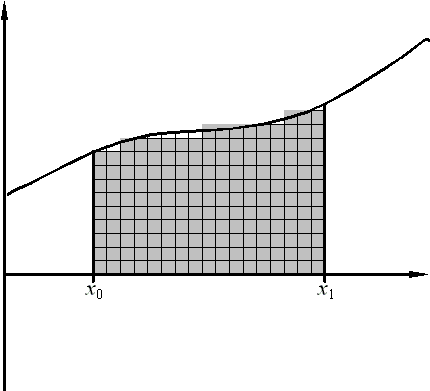
\includegraphics[width=0.4\textwidth]{graphics/manual}
	\caption{Manual method for determining the area below a graph. The grey squares are the ones which are by more than 50\% inside and thus are counted.}
	\label{fig:manual_integration}
\end{figure}


\subsection{Midpoint Rule}
The idea of the midpoint rule, which is also called \emph{rectangle method}, is to approximates the integral over an interval $[a, b]$ by calculating the area of a corresponding rectangle (see figure \ref{fig:midpoint_rule}). This rectangle has width $b-a$ and height $f(c)$ with $c=\frac{a+b}{2}$ being the midpoint. Thus the integral can be approximated with equation \ref{eq:midpoint_rule}. This rule is exact for polynomials with one degree, namely constant and linear functions. \cite{Wiki_Rectangle}

\begin{equation}
\int\limits_{a}^{b} f(x)\, dx \approx (b - a) \cdot f(c) = (b - a) \cdot f\!\left(\frac{a + b}{2}\right)
 \label{eq:midpoint_rule}
\end{equation}



\begin{figure}[hb]
\centering
\begin{minipage}{.45\textwidth}
  \centering
	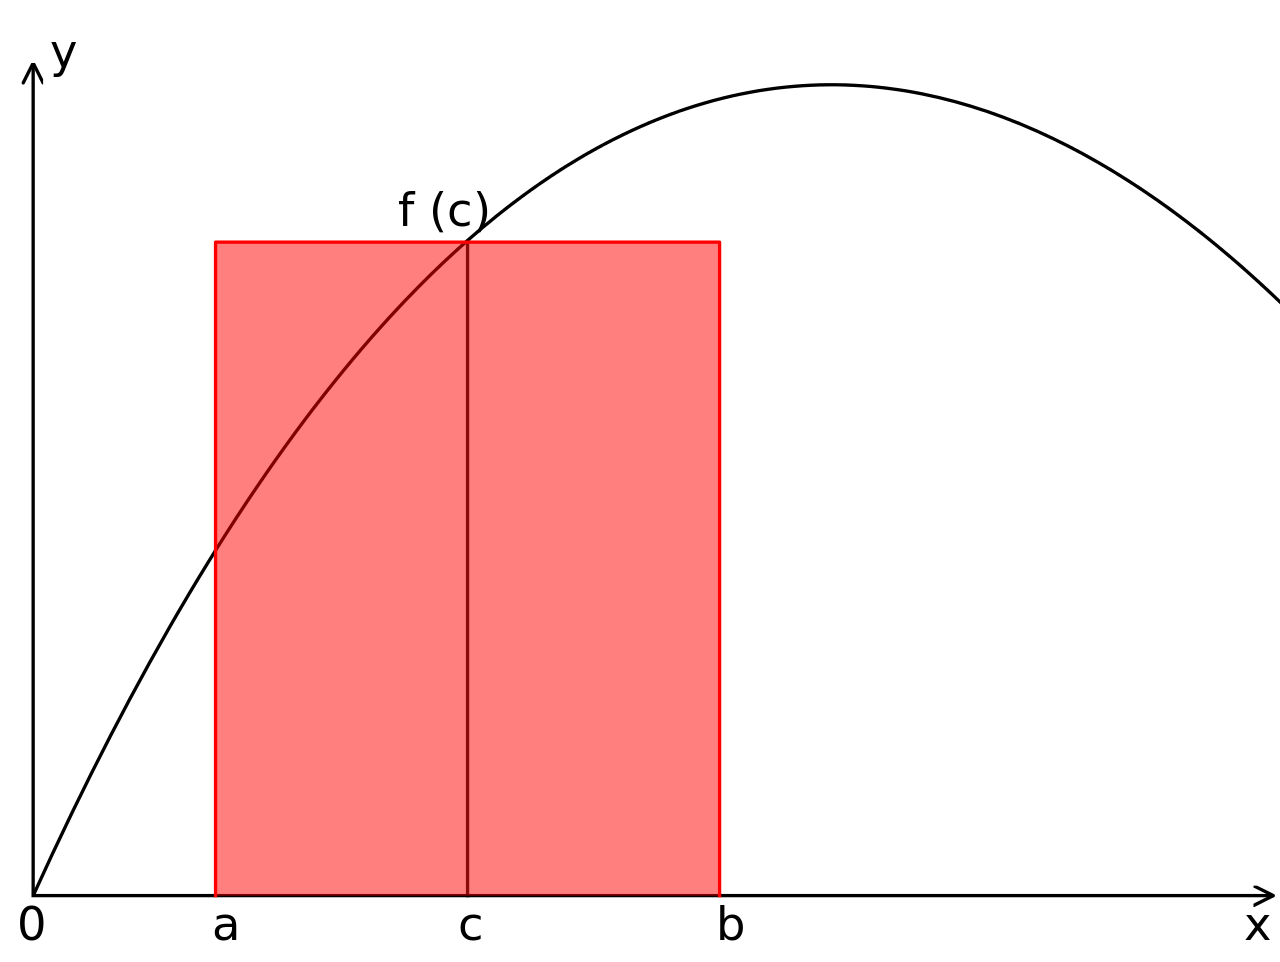
\includegraphics[width=0.9\textwidth]{graphics/midpoint.png}
	\caption{Midpoint Rule. Approximation of the integral by constructing a rectangle with height $f(c)$.}
	\label{fig:midpoint_rule}  
\end{minipage} \hspace{10px}
\begin{minipage}{.45\textwidth}
  \centering
  
\includegraphics[width=0.9\textwidth]{graphics/trapezoid3}
	\caption{Trapezoid Rule.\newline Approximation of the integral by constructing a trapezoid from $f(a)$ to $f(b)$. }
	\label{fig:trapez_integration}
\end{minipage}
\end{figure}

\subsection{Trapezoid Rule}
The trapezoid rule uses a similar concept as the Midpoint rule. It approximates the integral of a function by the area of a trapezoid as shown in figure \ref{fig:trapez_integration}. The trapezoid itself has base $h = b - a$ and sides equal to the values of the integrand at the two endpoints $a$ and $b$. Thus, the integral of a function can be approximated by equation \ref{eq:trapezoid_rule}. Again, this rule is exact for constant and linear functions but provides better approximations for functions of a higher degree, compared to the midpoint rule.

\begin{equation}
 \int_{a}^{b} f(x)\, dx \approx (b-a) \left[\frac{f(a) + f(b)}{2} \right]
 \label{eq:trapezoid_rule}
\end{equation}



\subsection{Composite Rules}
Although the previous rules are exact for constant and linear functions, one cannot expect neither the midpoint nor the trapezoid rule to give accurate results for polynomials of a higher degree over a large interval. Therefore the idea is to split the main interval into $n$ short sub-intervals and compute an approximation for each sub-interval as shown in figure \ref{fig:trapez_composite}. Summing up those partial results gives a better approximation of the integral over the whole interval. This is called the composite rule. \cite{Skokos2010}

\begin{figure}
\centering
  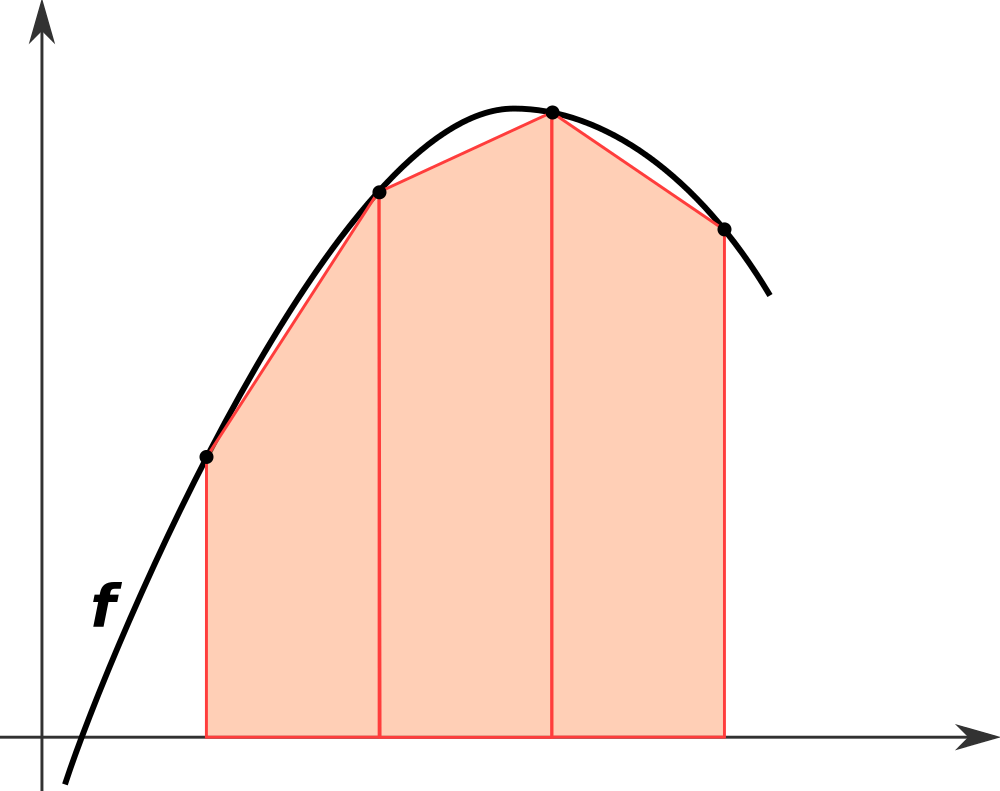
\includegraphics[width=0.5\textwidth]{graphics/trapez_composite.png}
	\caption{Trapezoid composite rule}
	\label{fig:trapez_composite}
\end{figure}


As $n$ gets larger, the intervals become smaller and the computation of the integral gets more accurate. This idea is the spirit of the definition of the Riemann integral and the limit of this approximation as n $\to \infty$ is defined and equal to the integral $\int_{a}^{b}\, f$, if this Riemann integral is defined. \cite{Wiki_Rectangle}

Comparing the midpoint and trapezoid rule, there are two advantages of the former one. First, there are less function evaluations needed to approximate the integral which can matter. Second it can be used more effectively for determining the integral near an integratable singularity since endpoints are not used, only a point inside the interval. \cite{Dalziel1998}

However, an analysis of Weidemann \cite{Weideman2002} shows that the trapezoid rule becomes extremely accurate when integrating periodic functions. He concludes that 'Using more sophisticated rules may not be worth the effort'.



\subsection{Simpsons's Rule}

The idea of the Simpson's rule is to use a parabola to approximate the integrand. This increases the accuracy of the approximation without a need to decrease the step size as much as it would be necessary with some lower order polynomial. The Simpson's rule provides exact results for any polynomial of degree three or less. The name of this rule comes from the English mathematician Thomas Simpson but since Kepler used similar formulas more than a century before, it sometimes is also called the Kepler's rule or Keplersche Fassregel. \cite{Wiki_Simpsons}

\begin{equation}
 \int_{a}^{b} f(x) \, dx \approx \tfrac{b-a}{6}\left[f(a) + 4f\left(\tfrac{a+b}{2}\right)+f(b)\right]
\label{eq:simpsons}
\end{equation}

Although this rule provides better results, approximating a function which is highly oscillatory or which lacks derivatives at certain points, the results may be still very poor. To increase the accuracy this function can also be used on sub-intervals and is then called the \emph{Composite Simpson's Rule}.

Formula \ref{eq:simpsons} is derived by evaluating the function at the two boundary points $a$ and $b$ of the interval, plus the midpoint $m = \frac{a+b}{2}$, see figure \ref{fig:Simpsons_rule2}. 

\begin{figure}[htbp]
	\centering
		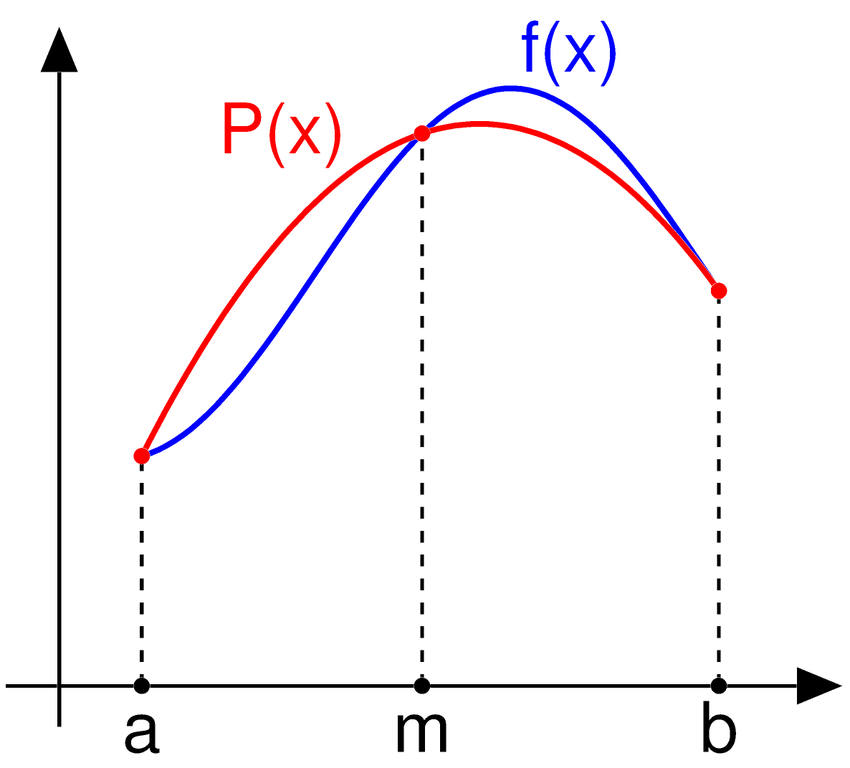
\includegraphics[width=0.40\textwidth]{graphics/simpsons2.png}
	\caption{Simpsons Rule. Using three points to interpolate a polynomial $p(x)$ in order to approximate $f(x)$.}
	\label{fig:Simpsons_rule2}
\end{figure}



\subsection{Newton-Cotes formulas}
When looking at the rules which are presented so far, it can be observed, that all rules have a general form, which is shown in equation \ref{eq:nq}. The points $x_i$ are always equally spaced and the rules only differ in the number of function points which are used for the approximation. Their corresponding weights $w_i$ are derived from Lagrange basis polynomials. An advantage of equal spacing is, that values can be reused which can minimizes the computational overhead.
\begin{equation}
\int_a^b f(x) \,dx \approx w_0 f(x_0) + w_1 f(x_1) + \dots + w_n f(x_n) = \sum_{i=0}^n w_i\, f(x_i)
\label{eq:nq}
\end{equation}

Equations \ref{eq:nq_mid}, \ref{eq:nq_trap} and \ref{eq:nq_simp} exemplary show the corresponding points $x_i$ and their weights.

\begin{equation}
\text{Midpoint:} \quad  x = \frac{a + b}{2}, \quad w = 1
\label{eq:nq_mid}
\end{equation}

\begin{equation}
\text{Trapezoid:} \quad x_0 = a, x_1 = b, \quad w_0 = w_1 = \frac{b-a}{2}
\label{eq:nq_trap}
\end{equation}

\begin{equation}
\text{Simpson's:}
\quad x_0 = a, x_1 = \frac{a+b}{2}, x_2 = b, 
\quad w_0 = w_2 = \frac{b-a}{6}, w_1 = 4 * \frac{b-a}{6}
\label{eq:nq_simp}
\end{equation}

There are two types of Newton-Cotes formulas, open and closed ones. While the former only uses the points in between the interval (for example the midpoint rule), the closed formulas (such as the Simpson's rule) also use the function values at the endpoints. Newton-Cotes formulas of any higher degree $n$ can be constructed as well. \cite{Wiki_Cotes} 


\subsection{Gaussian Quadrature}\label{sec:gauss_quad}
The main idea of the Gaussian quadrature is to not use equally spaced intervals at which the function is evaluated but to carefully choose the points $x_i$ and their weights to maximize accuracy. Thereby, the general form of the rule stays the same as for the Newton-Cotes rule (equation \ref{eq:nq}) but the $x_i$ and weights differ. There exist multiple forms of the Gaussian quadrature while the Gauss-Legende quadrature is the most known one. In general, the result of a rule which uses $n$ points is exact for polynomials of degree $2n-1$ or less. The Gauss-Legendre quadrature is by default defined over the interval $[-1, 1]$ so that an integral over an interval $[a, b]$ must be changed before the Gaussian quadrature rule can be applied. A change of interval can be done as shown in equation \ref{eq:interval}. However, there are other forms which are defined over other intervals. Although the computational overhead is slightly higher compared to the Newton-Cotes rules, the Gaussian quadrature rules are typically more accurate.  \cite{wiki:gauss}

Table \ref{tab:gauss_quad} shows some low order Gaussian-Legendre rules up to a degree of $5$.


\begin{equation}
\int_a^b f(x)\,dx = \frac{b-a}{2} \int_{-1}^1 f\left(\frac{b-a}{2}x + \frac{a+b}{2}\right)\,dx
\label{eq:interval}
\end{equation}


\newcommand{\specialcell}[2][c]{%
  \begin{tabular}[#1]{@{}c@{}}#2\end{tabular}}
\begin{table}[htbp]
\centering
\caption{Parameters for low order Gaussian-Legendre quadrature}
\begin{tabular}{|c|c|c|}
\hline
Number of points, $N$ & Points, $X_i$   & Weights, $w_i$   \\ \hline

1                   & 0               & 2               \\ \hline

2                   & 
$\pm \sqrt{\frac{1}{3}}$ & 1               \\ \hline

3                   
& \specialcell{$0$ \\ $\pm \sqrt{\frac{3}{5}}$}       
& \specialcell{$\frac{8}{9}$ \\ $\frac{5}{9}$} \\ \hline

4                   
& \specialcell{$\pm\sqrt{\tfrac{3}{7} - \tfrac{2}{7}\sqrt{\tfrac{6}{5}}}$
		\\ $\pm\sqrt{\tfrac{3}{7} + \tfrac{2}{7}\sqrt{\tfrac{6}{5}}}$}
& \specialcell{$\tfrac{18+\sqrt{30}}{36}$ \\ $\tfrac{18-\sqrt{30}}{36}$}  \\ \hline

5                   
& \specialcell{$0$ \\ $\pm\tfrac13\sqrt{5-2\sqrt{\tfrac{10}{7}}}$
		\\ $\pm\tfrac13\sqrt{5+2\sqrt{\tfrac{10}{7}}}$}
& \specialcell{$\tfrac{128}{225}$ \\ 
			$\tfrac{322+13\sqrt{70}}{900}$ \\ 
			$\tfrac{322-13\sqrt{70}}{900}$}  \\ \hline


\end{tabular}
\label{tab:gauss_quad}
\end{table}



% \subsection{Romberg Integration}

\subsection{Monte Carlo Method}
A method which does not use an approximation formula is the Monte Carlo method. Instead the integral is determined by randomly choosing $n$ points over the integration interval $[a, b]$. The integral is then approximated by the average over the function values at those random points (equation \ref{eq:montecarlo}).

\begin{equation}
\int_a^b f(x) \,dx \approx\frac {b-a}n \sum_{i=1}^n f(x_i)
\label{eq:montecarlo}
\end{equation}

The advantage of this approach is its easy implementation and extensibility, especially on multidimensional integrals. However, the computation time is higher compared to other approximation formulas. Moreover, Monte Carlo does not always provide $100\%$ correctness but in general the results will be correct. \cite{Robert2010, Judd2011}



\subsection{Multidimensional Integrals} 

When trying to estimate the value of multidimensional integrals, a distinction between cases of low and high dimensionality has to be made \cite{NAGlib}. Where the number of dimensionalities is lower than 4 or 5, one- dimensional methods, such as the ones mentioned above, may be applied to each dimension, according to some suitable strategy. However, special techniques are needed for integrals of higher dimensionality since the  number of evaluation rises very rapidly with the number of dimensions. Therefore non deterministic approaches such as the \emph{Monte-Carlo} method, which randomly chose the points at which the integrand is evaluated, can be used.
\section{Quadrature Methods} \label{routines}
This section will give an overview of routines available in numerical libraries to perform quadrature.  For reasons of simplicity only the GNU Scientific Library (GSL)\cite{GSL_Reference} and the NAG Numerical Library (NAGLib)\cite{NAGlib} are considered.
These routines are classified into three categories: one-dimensional, two-dimensional and multidimensional quadrature. Furthermore, another distinction between adaptive and non-adaptive routines can be made.

There exist general purpose routines for people who do not care about computation time or are not willing to do any analysis of the integral. However, if efficiency is needed, there exist a lot of methods which accept additional parameters for specifying peaks, singularities or other problematic points. Also desired relative and absolute error bounds for the approximation can be specified.

The final choice of a routine should be based amongst others on the type of interval, number of integrals, accepted error and available computation time.



\subsection{One-Dimensional Quadrature}
This section covers routines for numerical integration in one dimension. Both considered libraries are largely based on \emph{QUADPACK}, a Fortran library for numerical integration of one-dimensional functions by Piessens et al.\cite{quadpack}. There are nine routines for automatic quadrature included in QUADPACK which are described in the scope of this section.

The naming conventions for the algorithms in QUADPACK use the following naming scheme:
\begin{itemize}[noitemsep]
\item[Q] - Quadrature routine
\newline
\item[N] - Non-adaptive integrator
\item[A] - Adaptive integrator
\newline
\item[G] - General integrand (user-defined)
\item[W] - Weight function with integrand
\newline
\item[S] - Singularities can be more readily integrated
\item[P] - Points of special difficulty can be supplied
\item[I] - Infinite range of integration
\item[O] - Oscillatory weight function, cos or sin
\item[F] - Fourier integral
\item[C] - Cauchy principal value
\end{itemize}

Since the GSL uses a similar naming scheme (\emph{gsl\_integration\_} + *quadpack\_algorithm\_name*) the function names will not be stated separately for the GSL. 

\subsubsection{QNG}
QNG calculates an approximation to the integral of a function over a finite interval. It is a simple and non-adaptive routine and thus only recommended for smooth functions which neither have singularities, nor height peaks nor oscillate strongly. Depending on the desired accuracy the routine uses a 10-point, 21-point, 43-point or 87-point Gaussian rule. This is the only non-adaptive automatic integrator of QUADPACK. \cite{quadpack, GSL_Reference}

NAGLib name: nag\_quad\_1d\_fin\_smooth (d01bdc) \cite{nag_d01bdc}



\subsubsection{QAG}
QAG is a simple globally adaptive integrator which uses 30-point and 61-point Gauss-Kronrod rules. The integration region is divided into subintervals, and on each iteration the subinterval with the largest estimated error is bisected. As this function is based on integration rules of high order, it is especially suitable for non-singular oscillating integrands. \cite{nag_d01skc, quadpack, GSL_Reference}

NAGlib name: nag\_1d\_quad\_osc\_1 (d01skc) \cite{nag_d01skc}



\subsubsection{QAGS}
The QAGS routine is one of two general purpose routines, which are suitable for use without further analysis of the integrand. While this one is for integration over a finite interval, QAGI is the corresponding one for integration over an infinite interval. QAGS is a globally adaptive routine based on 21-point Gauss-Kronrod quadrature in connection with extrapolation. This routine is suitable as a general purpose integrator, and can be used when the integrand has singularities, especially when these are of algebraic or logarithmic type. \cite{quadpack, GSL_Reference, nag_d01sjc}

NAGlib name: nag\_1d\_quad\_gen\_1 (d01sjc) \cite{nag_d01sjc}

Another general purpose implementation, which is included in the NAGlib (nag\_quad\_1d\_fin\_gonnet\_vec (d01rgc)) and is similar but differs in how the evaluation error is estimated and in how singularities are treated. \cite{nag_d01rgc}



\subsubsection{QAGP}
QAGP is a modified version of the QAGS routine which allows the user to supply additional \emph{breakpoints}, points at which the function is difficult, such as internal singularities, discontinuities and other difficulties of the integrand function. By providing these breakpoints, the routine is less computational expensive than the original QAGS routine. \cite{quadpack, GSL_Reference, nag_d01slc}

NAGlib name: nag\_1d\_quad\_brkpts\_1 (d01slc) \cite{nag_d01slc}



\subsubsection{QAGI}
QAGI is the second general purpose routine which is the only routine for infinite intervals. Internally the infinite interval is mapped onto the semi-open interval $(0,1]$ using a transformation similar to equation \ref{eq:interval}. After that a similar approach as in QAGS is used, except with 15-point rather than 21-point Gauss-Kronrod quadrature. \cite{quadpack, GSL_Reference, nag_d01smc}

NAGlib name: nag\_1d\_quad\_inf\_1 (d01smc) \cite{nag_d01smc}


\subsubsection{QAWO} QAWO is designed for integrands with an oscillatory 
factor, $\sin(\omega x)$ or $\cos(\omega x)$. Internally an adaptive 
subdivision scheme is used, which is a modification of the one in QAGS. Thus 
this routine can also deal with singularities. \cite{GSL_Reference, quadpack, 
nag_d01snc}

NAGlib name: nag\_1d\_quad\_wt\_trig\_1 (d01snc) \cite{nag_d01snc}



\subsubsection{QAWF}
QAWF calculates an approximation to the sine or the cosine transform of a function over a semi-infinite interval using a Fourier transform. The integral is computed using the QAWO algorithm over each of the subintervals.\cite{GSL_Reference, quadpack, nag_d01ssc}

NAGlib name: nag\_1d\_quad\_inf\_wt\_trig\_1 (d01ssc) \cite{nag_d01ssc}



\subsubsection{QAWS}
QAWS is an adaptive integrator which integrates a function of the form $\int_a^b g(x) w(x) \mathrm{d}x$, where the weight function $w$ may have algebraic-logarithmic singularities at the end-points $a$ and/or $b$\cite{quadpack}. In order to work efficiently the algorithm requires a precomputed table of Chebyshev moments which are used on all sub-intervals which have a or b as one of their end-points. On the other sub-intervals Gauss–Kronrod (7–15 point) integration is carried out.\cite{GSL_Reference, nag_d01spc}.

NAGlib name: nag\_1d\_quad\_wt\_alglog\_1 (d01spc) \cite{nag_d01spc}


\subsubsection{QAWC}
QAWC computes the Cauchy principal value of the integral of $f(x)$ over $(a,b)$, with a singularity at c. \cite{quadpack}
\begin{equation}
I = \int_a^b dx f(x) / (x - c) \mathrm{d}x
\label{eq:qawc}
\end{equation}
A globally adaptive bisection algorithm ensures that subdivisions do not occur at the singular point x = c. If  a sub-interval contains the point x = c or is close to it then a special 25-point modified Clenshaw-Curtis rule is used to control the singularity. Further away from the singularity the algorithm uses an ordinary 15-point Gauss-Kronrod integration rule. \cite{GSL_Reference}

NAGlib name: nag\_1d\_quad\_wt\_cauchy\_1 (d01sqc) \cite{nag_d01sqc}



\subsubsection{Gauss-Quadrature}
The fixed-order Gauss-Legendre integration routines, whose rules are presented in more detail in section \ref{sec:gauss_quad}, provide fast integration of smooth functions with known polynomial order over a finite interval. Both libraries provide a method for approximating an integral by a n-point Gauss-Legendre rule which is exact for polynomials up to an order of $2*n-1$. Unlike the other numerical integration routines which are presented before, these routines do not accept absolute or relative error bounds. \cite{nag_d01tac, GSL_Reference} \newline
The NAGlib also provides formulae for semi-infinite intervals (Gauss–Laguerre, rational Gauss) and infinite interval (Gauss–Hermite). \cite{nag_d01tac}



\subsubsection{Data Values}
The function nag\_1d\_quad\_vals (d01gac)\cite{nag_d01gac} is part of the NAGlib and integrates functions which are defined by data values only. The function to integrate needs to be specified at four or more points over the whole range. The points can be unequally spaced but should be in either ascending or descending order. 




\subsection{Two-Dimensional Quadrature}
The value of a two-dimensional integral can be determined by first integrating along one axis and then a along another. Additionally, NAGlib provides one specialized function, nag\_quad\_2d\_fin (d01dac) \cite{nag_d01ac}, to evaluate a definite double integral, such as the one in equation \ref{eq:double} where a and b are constants and $\phi_1{y}$ and $\phi_2{y}$ are functions of the variable y. Both integrals, the inner and the outer one, are then evaluated with the method described by Patterson \cite{Patterson1967} of 'the optimum additions of points to quadrature formulae'.

\begin{equation}
	\int_a^b \int_{\phi_1{y}}^{\phi_2(y)} f(x,y)  \, \mathrm{d}xy = \int_a^b F(y) \, \mathrm{d}y \, \quad
	\text{where} \quad F(y) = \int_{\phi_1{y}}^{\phi_2(y)} f(x,y)\, \mathrm{d}x
\label{eq:double}
\end{equation}



\subsection{Multidimensional Quadrature}
This sections gives a short overview of the routines for multidimensional quadrature which are provided in the two considered numerical libraries. The routines and their general idea will only be mentioned briefly since the interested reader needs to become familiar with more specific or complex concepts such as number theoretic transformations, hypercubes, sparse grids, simplexes, etc. which are beyond the scope of this work.


\subsubsection{Multidimensional Quadrature in GSL}
There are no native routines for multidimensional quadrature included in the GSL. However, there exists a third-party package by Steven G. Johnson which provides adaptive multidimensional integration as extension. Two algorithms are provided.

The first recursively partitions the integration domain into smaller subdomains and applies the same integration rule to each, until convergence is achieved. 'This algorithm is best suited for a moderate number of dimensions (say, $< 7$), and is superseded for high-dimensional integrals by other methods (e.g. Monte Carlo variants or sparse grids).'

The second routine repeatedly doubles the degree of the quadrature rules until convergence is achieved. 'This algorithm is often superior to h-adaptive integration for smooth integrands in a few ($<=3$) dimensions, but is a poor choice in higher dimensions or for non-smooth integrands.' \cite{Johnson}

\subsubsection{Multidimensional Quadrature in NAGlib}
The NAGlib provides seven methods for determining the value of a multidimensional integral which are outlined below:

\begin{itemize}
\item nag\_quad\_md\_sgq\_multi\_vec (d01esc) \cite{nag_d01esc} \newline
Uses sparse grids to estimate a vector $F$ of integrals over the unit hypercupe, given the vector of $f(x)$. This routine is feasible  for estimating integrals of high dimensions $d\sim O(100)$

\item nag\_quad\_md\_gauss (d01fbc) \cite{nag_d01fbc} \newline
This function uses Gaussian weights and abscissas to compute the value of a multidimensional integral over a hyper-rectangle. The number of dimensions may be anything between 1 and 20.

\item nag\_quad\_md\_sphere (d01fdc) \cite{nag_d01fdc} \newline
An approximation to a definite integral in up to 30 dimensions is computed by using the method of Sag and Szekers. The integration region is an n-sphere which can also be transformed to an n-cube.

\item nag\_quad\_md\_numth\_vec (d01gdc) \cite{nag_d01gdc} \newline
Uses a number theoretic approach to approximate an multidimensional definite integral in up to 20 dimensions. The result depends on the sequence of random numbers which is generated.

\item nag\_quad\_md\_simplex (d01pac) \cite{nag_d01pac} \newline
This function integrates a multidimensional integral by computing a sequence of approximations over a n-dimensional simplex.

\item nag\_multid\_quad\_adapt\_1 (d01wcc) \cite{nag_d01wcc} \newline
Estimates the integral over a hyper-rectangle with constant limits. It repeatedly subdivides each hyper-rectangle into smaller ones and applies a seventh-degree rule to it.

\item nag\_multid\_quad\_monte\_carlo\_1 (d01xbc) \cite{nag_d01xbc} \newline
Uses a Monte-Carlo method to approximate the integral of a function over a hyper rectangle. In the beginning the function subdivides the integration region into smaller sub-regions and estimates the integral and variance of each sub-region. The routine stops when desired accuracy has been reached or too many integral evaluations are required in the next cycle. Since this function relies on random numbers, each run may return different results.
		
\end{itemize}






\section{Summary}

This work shows several ways how to estimate an integral numerically. This is 
desired if either the integrand is partially unknown, there is no 
antiderivative or its computation is too expensive. At this point numerical 
algorithms provide an easier and approximated solution of the integral.

In the first part, the most important concepts are presented. The basic idea 
of these approaches is to evaluate the integrand at a finite set of points 
and then to sum these values with addition of a weighting function. If the 
function to be integrated is of a low polynomial degree, an exact solution 
can be obtained by the Gaussian quadrature which only requires n points to 
approximate a polynomial of degree $2n-1$. However, if the function has a 
high degree, oscillates or contains singularities, other concepts are needed. 
This often results in more function evaluations and can become expensive 
again. 

A variant to approximating the integral of a function in one step is to subdivide the interval into smaller intervals and determine the integral as a sum of all sub intervals. Especially on periodic functions, the composite midpoint rule becomes extremely accurate. The values of multidimensional intervals can also be determined by using a one-dimensional method in each dimension. This approach is only suitable for low dimensions since the number of evaluations rises exponentially with increasing degree. A technique which evaluates an integral at a random number of points are Monte-Carlo methods.

The second part gives an overview of the routines implemented in numerical 
libraries. As example libraries the Gnu Scientific Library and the library of 
the Numerical Algorithms Group are considered. In the one-dimensional case 
they both mostly rely on QUADPACK, a Fortran library for numerical 
integration of one-dimensional integrals. QAGS and QAGI are two general 
purpose routine which can be used without further analysis of the integrand 
while the former is for the use over finite intervals and the latter for 
infinite intervals. However, there are routines specialized in integrals of functions 
which have singularities or are strongly oscillating. Using such a 
specialized function will be less expensive in most cases since fewer 
conditions need to be checked.

Although the GSL does not natively include methods for multidimensional integration, 
there exists an extension for that purpose. NAGlib provides routines for 
multidimensional integration over hyper rectangles and simplexes, n-cubes and 
n-spheres innately. Moreover, a routine which uses a Monte-Carlo method is 
included as well. With the returned absolute or relative error assumptions of 
the accuracy can be made.






\section{Appendix}
Tutorial exercises.

\begin{equation}
\int_0^\pi \sin(x) \, dx
\label{eq:}
\end{equation}

\begin{figure}[h]
	\centering
		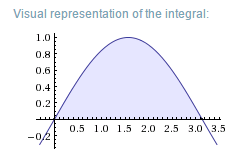
\includegraphics{graphics/intsinx.png}
	\caption{$sin(x)$}
	\label{fig:intsinx}
\end{figure}


\subsection{Integration with the 'simple rules'}
\begin{enumerate}
	\item Estimate the exact solution to the integral
	\item Use the Midpoint, Trapezoid and Simpson's rule to approximate the integral.
	\item Use the composite trapezoid rule for two and four intervals to approximate the integral.
\end{enumerate}


\subsubsection{Solution}
$a = 0, b = \pi$

\begin{enumerate}
	\item Solving the integral:
	\begin{equation}
\int_0^\pi \sin(x) \, dx = -\cos(x) \Big|_{x=0}^{x=\pi} = 2
\label{sol:int}
\end{equation}
	
	\item Solution for midpoint (\ref{sol:midpoint}), trapezoid (\ref{sol:trapezoid_rule}) and simpson's (\ref{sol:simpsons}) rule to approximate the integral.	
	
	\begin{equation}
\int\limits_{a}^{b} f(x)\, dx \approx (b - a) \cdot f\!\left(\frac{a + b}{2}\right) 
= (\pi) \cdot \sin{\!\left(\frac{\pi}{2}\right)} = \pi
 \label{sol:midpoint}
\end{equation}
	
	\begin{equation}
 \int_{a}^{b} f(x)\, dx \approx (b-a) \left[\frac{f(a) + f(b)}{2} \right] = \pi * \frac{0}{2} = 0
 \label{sol:trapezoid_rule}
\end{equation}
	
	
	\begin{equation}
 \int_{a}^{b} f(x) \, dx \approx \tfrac{b-a}{6}\left[f(a) + 4f\left(\tfrac{a+b}{2}\right)+f(b)\right]
 = \tfrac{\pi}{6}\left[4 \sin \left(\tfrac{\pi}{2}\right)\right] =  \frac{2 \pi}{3} \approx 2.094
\label{sol:simpsons}
\end{equation}
	
	
	\item Application of the composite trapezoid rule on two intervals:
	
	$a_1 = 0, b_1 = a_2 = \pi / 2, b_2 = \pi$
	
	\begin{equation}
 \int_{0}^{\frac{\pi}{2}} \sin(x)\, dx \approx \frac{\pi}{2} \left[\frac{\sin(0) + \sin(\frac{\pi}{2})}{2} \right] = \frac{\pi}{4}
 \label{sol:trleft}
\end{equation}

\begin{equation}
 \int_{\frac{\pi}{2}}^{\pi} \sin(x)\, dx \approx \frac{\pi}{2} \left[\frac{\sin(\frac{\pi}{2}) + \sin(\pi)}{2} \right] = \frac{\pi}{4}
 \label{sol:trright}
\end{equation}

\begin{equation}
 \int_{0}^{\frac{\pi}{2}} \sin(x)\, dx + \int_{\frac{\pi}{2}}^{\pi} \sin(x)\, dx \approx \frac{\pi}{2} = 1.571
 \label{sol:add}
\end{equation}

\begin{figure}
	\centering
		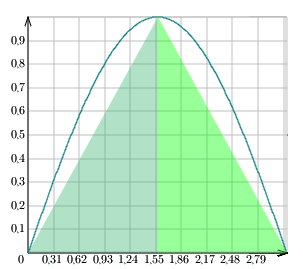
\includegraphics[width=0.50\textwidth]{graphics/trapezn2.png}
	\caption{Trapezoid rule for n = 2}
	\label{fig:trapezn2}
\end{figure}


	
	\item Application of the composite trapezoid rule on four intervals:
	
	\begin{equation}
 \int_0^\pi \sin(x) \, dx = 
 \int_{0}^{\frac{\pi}{4}} \sin(x)\, dx 
+\int_{\frac{\pi}{4}}^{\frac{\pi}{2}} \sin(x)\, dx 
+ \int_{\frac{\pi}{2}}^{\frac{3\pi}{4}} \sin(x)\, dx 
+\int_{\frac{3\pi}{4}}^{\frac{\pi}{2}} \sin(x)\, dx 
= \dots \approx 1.8961
\end{equation}
	
\begin{figure}
	\centering
		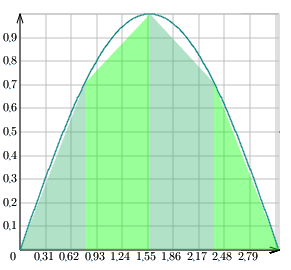
\includegraphics[width=0.50\textwidth]{graphics/trapezn4.png}
	\caption{Trapezoid rule for n=4}
	\label{fig:trapezn4}
\end{figure}	
	
\end{enumerate}


\subsection{Gaussian Quadrature}
Transform the interval from $[0, \pi]$ to $[-1, 1]$ and apply the Gaussian quadrature rule for $n=2$

\subsubsection{Interval Transformation}

The formula from section \ref{sec:gauss_quad}

\begin{equation}
\int_a^b f(x)\,dx = \frac{b-a}{2} \int_{-1}^1 f\left(\frac{b-a}{2}x + \frac{a+b}{2}\right)\,dx
\end{equation}

Applied to our integral

\begin{equation}
\int_0^\pi \sin(x) \, dx = \frac{\pi}{2} \int_{-1}^1 \sin\left(\frac{\pi}{2}x + \frac{\pi}{2}\right)\,dx
\end{equation}

\subsubsection{Application of the Gaussian Quadrature Rule}

The tranforme interval

\begin{equation}
\frac{\pi}{2} \int_{-1}^1 \sin\left(\frac{\pi}{2}x + \frac{\pi}{2}\right)\,dx
\end{equation}

The Gaussian two-point rule:
$$\int_{-1}^1 f(x) \, dx \approx f(- \frac{1}{\sqrt{3}} ) + f( \frac{1}{\sqrt{3}} )$$

Deployed:

\begin{equation}
\frac{\pi}{2} \int_{-1}^1 \sin\left(\frac{\pi}{2}x + \frac{\pi}{2}\right)\,dx
= \frac{\pi}{2} \left( \int_{-1}^1 f'(x) \, dx \right)
\approx  \frac{\pi}{2} \left( f'(- \frac{1}{\sqrt{3}} ) + f'( \frac{1}{\sqrt{3}} ) \right)
\end{equation}

\begin{equation}
f'(x) = \sin\left(\frac{\pi}{2}x + \frac{\pi}{2}\right)
\end{equation}

\begin{equation}
f'(\pm \frac{1}{\sqrt{3}}) = 0.6162
\end{equation}

\begin{equation}
=> \frac{\pi}{2} \int_{-1}^1 \sin\left(\frac{\pi}{2}x + \frac{\pi}{2}\right)\,dx
\approx \frac{\pi}{2} * 0.6162 = 1,936
\end{equation}


\newpage

\subsection{Comparison}
Compare the results.

\subsubsection{Solution}
\begin{itemize}
	\item [Exact: ] 2
	\item [Midpoint: ] $\pi$
	\item [Trapezoid n = 1:] 0
	\item [Trapezoid n = 2: ] $1.571$
	\item [Trapezoid n = 4:] $1.896$
	\item [Simpson's: ] $2.094$
	\item [Gaussian n = 1: ] $1.936$
\end{itemize}

The trapezoid rule for n = 1 has the worst result. However, one can see how the results get better when the interval is subdivided and more points are considered. This fact is also clearly visible when viewing the corresponding figures. The Simpson's rule is close but the Gaussian rule provides the best result while only using two points. The midpoint rule uses only one point and thus provides also a bad approximation but one can image that its performance increases when the interval is subdivided as with the trapezoid rule.






% \bibliographystyle{chicago}

\printbibliography

\end{document}

